\section{Especificaciones Formales y VDM++}
\subsection{VDM++}
La Vienna Development Method (VDM) es uno de los métodos formales más antiguos y establecidos orientados a modelos para el desarrollo de sistemas y software en entornos computacionales. Este método utiliza un conjunto de lenguajes rigurosamente fundamentados en la matemática para representar y analizar modelos de sistemas en las primeras fases del diseño. Esto permite evaluar las propiedades clave del sistema antes de realizar compromisos significativos relacionados con la implementación. Gracias a la construcción y análisis de estos modelos, es posible identificar áreas donde las especificaciones informales del sistema pueden ser incompletas o ambiguas, lo que proporciona una mayor confianza en que la implementación final respetará propiedades fundamentales, como la seguridad y la protección \cite{smith2021}.

\subsection{Definición de Clases}
En VDM++, las clases son bloques fundamentales que encapsulan tanto datos como operaciones. Las clases se definen mediante la especificación de sus atributos (variables de instancia) y métodos (funciones y operaciones). Cada clase también puede incluir invariantes que describen condiciones que deben mantenerse verdaderas a lo largo de la vida de la clase \cite{fitzgerald2009}.

\begin{figure}[h]
    \centering
    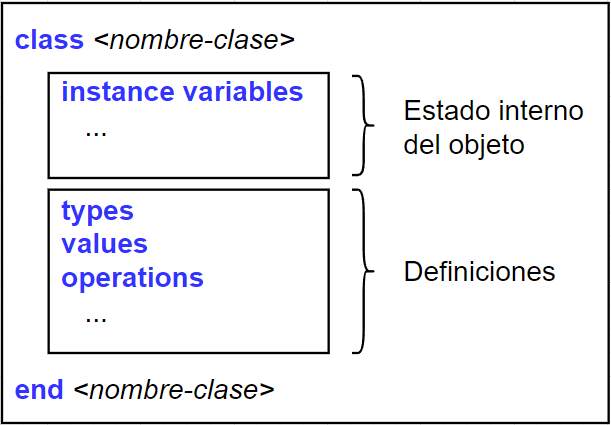
\includegraphics[width=0.5\textwidth]{Recursos/estructura_clases_vdm.png}
    \caption{Estructura básica de formalización de clases en VDM++}
\end{figure}

\subsection{Tipos}
VDM++ soporta una amplia variedad de tipos, tanto básicos como estructurados. Entre los tipos básicos se incluyen enteros, reales, booleans, y caracteres, mientras que los tipos estructurados pueden ser secuencias, conjuntos, y tuplas. Además, los tipos definidos por el usuario permiten una mayor flexibilidad y robustez en la modelización de sistemas complejos \cite{woodcock1996}.

\begin{figure}[h]
    \centering
    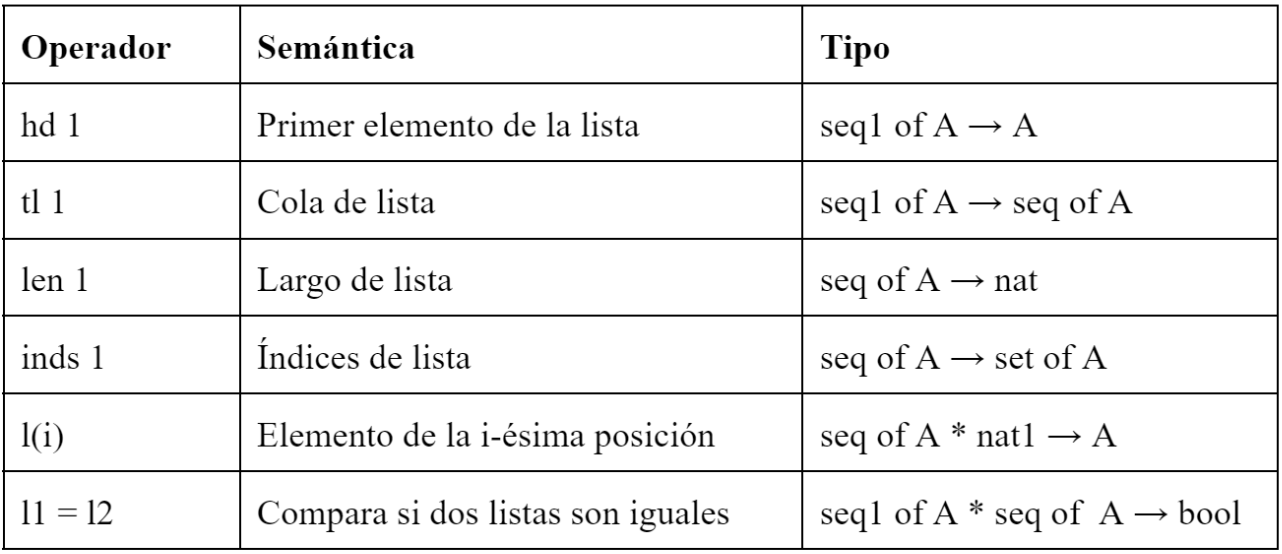
\includegraphics[width=0.5\textwidth]{Recursos/tipos_variables_vdmpp.png}
    \caption{Operaciones Formales de tipo secuencia en VDM++}
\end{figure}
\newpage
\subsection{Expresiones}
Las expresiones en VDM++ están definidas de manera formal utilizando operadores matemáticos y lógicos. Estas expresiones pueden ser aritméticas, booleanas o relacionales, y se emplean para definir propiedades del sistema, como las precondiciones y postcondiciones de funciones y operaciones, así como las invariantes de las clases \cite{fitzgerald2009}.



